\documentclass[a4paper,rep]{thesisby}

\usepackage[utf8]{inputenc}
\usepackage[english, russian]{babel}
\usepackage[hidelinks]{hyperref}
\hypersetup{
    allcolors=black
}

\usepackage{lastpage} % для указания общего числа страниц
\usepackage{amsmath} % для математических формул
\usepackage{IEEEtrantools} % для создания многострочных математических формул
\usepackage{commath} % для знака модуля

% для подсчёта числа источников литературы,
% но работает только после второй сборки
\usepackage{totcount}
\newtotcounter{citenum}
\def\oldcite{}
\let\oldcite=\bibcite
\def\bibcite{\stepcounter{citenum}\oldcite}

\newcommand{\No}{\textnumero}

\begin{document}

\begin{titlepage}

\begin{center}
{
Министерство образования и науки Российской Федерации\\
Федеральное государственное автономное образовательное учреждение\\
высшего образования\\
<<Санкт-Петербургский политехнический университет Петра Великого>>
}
\end{center}
\vspace{0.5cm}

\hspace{-15mm}
\begin{tabular}{lcr} 
{
	\begin{tabular}[t]{l}
		УДК 12345\\
		\No{12345} \\
		Инв. \No{12345} \\
	\end{tabular}
} & \hspace{40mm} & {
	\begin{tabular}[t]{l}
		У Т В Е Р Ж Д А Ю \\
		Зав. НИЛ <<Математическая биология\\
		и биоинформатика>>, ИПММ\\
		ФГАОУ ВО <<СПбПУ>>,\\
		д.б.н. \\
		\underline{\hspace{4cm}} М.~Г.~Самсонова\\
		<<\underline{\hspace{1cm}}>> \underline{\hspace{3cm}} 2015 г.
	\end{tabular}
}\\
\end{tabular}
\vspace{2cm}



\begin{center}
{
ОТЧЕТ\\
О НАУЧНО-ИССЛЕДОВАТЕЛЬСКОЙ РАБОТЕ\\
\vspace{3mm}
по теме:\\
<<Развитие метода разностной эволюции для поиска параметров математических моделей. Анализ эффективности различных методов>>\\
}
\end{center}

\vspace{3cm}


\hspace{15mm}
\begin{tabular}{ll}
{
	\hspace{60mm}
}&{
	\begin{tabular}[t]{l}
		Выполнил студент гр. \No{53601/4}\\
		{}\\
		\underline{\hspace{2cm}} А.~В.~Свичкарев\\
		<<\underline{\hspace{1cm}}>> \underline{\hspace{3cm}} 2015 г.
	\end{tabular}
}\\
{
	{}
}&{
}\\
{
	{}
}&{
	\begin{tabular}[t]{l}
		Руководитель НИР, к.б.н., в.н.с \qquad\\
		{}\\
		\underline{\hspace{2cm}} К.~Н.~Козлов\\
		<<\underline{\hspace{1cm}}>> \underline{\hspace{3cm}} 2015 г.
	\end{tabular}
}\\
\end{tabular}
\vspace{16mm}

\begin{center}
 Санкт--Петербург  2015
\end{center}

\end{titlepage}


\clearpage

\chapter*{РЕФЕРАТ}

% регистрируем счётчики в системе totcounter
\regtotcounter{totalcount@figure}
\regtotcounter{totalcount@table}       % Если поставить в преамбуле то ошибка в числе таблиц
\regtotcounter{TotPages}               % Если поставить в преамбуле то ошибка в числе страниц
\regtotcounter{citenum}

Отчёт \formbytotal{TotPages}{страниц}{а}{ы}{},
1 часть,
\formbytotal{totalcount@figure}{рисун}{ок}{ка}{ков},
\formbytotal{totalcount@table}{таблиц}{а}{ы}{}.
\formbytotal{citenum}{источник}{}{а}{ов}.
\bigskip

Ключевые слова:
МЕТОД ПОЛНОСТЬЮ ПАРАЛЛЕЛЬНОЙ РАЗНОСТНОЙ ЭВОЛЮЦИИ,
ИНТЕРПРЕТАТОР ЯЗЫКА R,
МЕЖПРОЦЕССОРНОЕ ВЗАИМОДЕЙСТВИЕ,
СИНХРОНИЗАЦИЯ ОБРАБОТКИ ДАННЫХ.

Целью работы является развитие
метода ППРЭ,
улучшение взаимодействия между методом оптимизации
и функционалом качества.

Учитывая, что для решения задачи
минимизации произвольной целевой функции
не существует универсального алгоритма,
разработка и усовершенствование
методов их решения остаётся актуальной задачей.

В данной работе был спроектирован
способ увеличения производительности
метода разностной эволюции
для поиска параметров математических моделей.
Была получена реализация
с применением распараллеливания вычислений
благодаря увеличению числа интерпретаторов.
Проведено тестирование быстродействия
новой реализации и показана эффективность улучшения.


\clearpage

\tableofcontents
\clearpage

\chapter*{ОБОЗНАЧЕНИЯ И СОКРАЩЕНИЯ}
\addcontentsline{toc}{section}{ОБОЗНАЧЕНИЯ И СОКРАЩЕНИЯ}

\textbf{РЭ} --- разностная эволюция (Differential Evolution);

\textbf{DEEP, ППРЭ} --- полностью параллельная разностная эволюция (Differential Evolution Entirely Parallel);

\textbf{Интерпретатор} --- программа, выполняющая пооператорный (покомандный, построчный) анализ, обработка и тут же выполнение исходной программы или запроса.

\textbf{Ассинхронная очередь задач} --- 
паттерн в программировании,
представляющий структуру,
содержащую переиспользуемые
потоки параллельного исполнения
для вычислительных задач.

\clearpage

\chapter*{ВВЕДЕНИЕ}
\addcontentsline{toc}{section}{ВВЕДЕНИЕ}

Проведение вычислительного эксперимента
в большинстве случаев обходится значительно дешевле,
чем проведение соответствующего эксперимента
над реальным биологическим объектом.
Именно поэтому важно развивать новые подходы в моделировании.

Важным классом программ для моделирования
являются пакеты программ
для решения обратной задачи математического моделирования.
Постановка задачи ставится
как минимизация функционала качества
при условии ограничений на параметры.

Для обратной задачи чаще всего модель известна,
но не известны некоторые параметры модели.
Задача заключается в нахождение этих параметров,
например, из данных уже проведённых экспериментов,
либо постановки дополнительных экспериментов,
называемых активным наблюдением.

Методы оптимизации можно классифицировать
в соответствии с задачами оптимизации
на локальные методы,
которые сходятся к локальному экстремуму целевой функции
(в случае унимодальной функции,
экстремум единственный и одновременно
является глобальным экстремумом)
и глобальные методы,
которые стремятся к выявлению
глобальных тенденций поведения целевой функции
и поиску глобального экстремума.

Метод полностью параллельной разностной эволюции
(далее ППРЭ, DEEP) \cite{Kozlov11, Kozlov13}
является модификацией стохастического метода оптимизации,
предложенного в \cite{Storn95}.
DEEP представляет из себя эффективный метод
решения обратной задачи математического моделирования,
а именно модификация глобального стохастического метода
и метод оптимального наискорейшего спуска
для поиска минимума функционала качества
на основе необходимого условия стационарности первого порядка.
Это значит, что он способен недетерминированно
(т.е. с использованием вероятностных методов)
находить экстремум для многоэкстремальных целевых функций
только с использованием вычисления целевой функции
в точках приближения без требования вычисления частных производных функции.

Целью работы является развитие метода ППРЭ,
улучшение взаимодействия между
методом оптимизации и функционалом качества,
что приводит к увеличению производительности.

Математические модели в биоинформатике
в большинстве случаев создаются
в таких компьютерных системах расчетов
как R, MATLAB, Octave и других.
Нахождение параметров в таких моделях
требует многократного вычисления решений,
что влечет большие накладные расходы на запуск
того или иного интерпретатора.
Однако, интерпретатор может быть встроен в программу ППРЭ,
что позволит запускать нужное число копий один раз,
и, тем самым сократить время вычислений, для некоторых задач в разы.

Таким образом,
развитие методов решения обратной задачи математического моделирования
и эффективное распараллеливание существующих решений
является важным для исследований системной биологии.


\clearpage

\setcounter{figure}{0} \setcounter{table}{0} \setcounter{equation}{0}
\chapter*{ОСНОВНАЯ ЧАСТЬ}
\addcontentsline{toc}{section}{ОСНОВНАЯ ЧАСТЬ}

\setcounter{figure}{0} \setcounter{table}{0} \setcounter{equation}{0}
\chapter*{ОСНОВНАЯ ЧАСТЬ}
\addcontentsline{toc}{section}{ОСНОВНАЯ ЧАСТЬ}

\section*{Теория метода DEEP}
\addcontentsline{toc}{subsection}{Теория метода DEEP}

Ниже приведено описание оригинального метода разностной эволюции
и его модификации DEEP.

Разностная эволюция (РЭ) ---
стохастический итерационный алгоритм минимизации,
предложенный Сторном и Прайсом в 1995 г.~\cite{Storn95}.

Метод оперирует случайно сгенерированными векторами параметров,
называемых индивидами. 
Под вектором понимается точка n-мерного пространства
из области определения целевой функции,
которую требуется минимизировать.
Множество индивидов называется популяцией.
Одна итерация популяции РЭ называется поколением.
Первое поколение генерируется случайным образом.
Новое поколение создаётся
по заданной схеме из индивидов текущего поколения.

Идея генерации нового поколения в оригинальном алгоритме
заключается в следующем.
Для каждого индивида текущего поколения
выбираются случайным образом 3 другие индивида
из поколения и вычисляется мутантный вектор по формуле:

\begin{equation} \label{mutant}
    v = v_1 + S \cdot (v_2 - v_3),
\end{equation}

где \begin{math}S\end{math} некоторая положительная константа масштабирования.

Производится операция скрещивания мутантного вектора с исходным,
замещением некоторых координат значениями из исходного вектора.
Полученный вектор называется пробным вектором.
Если значение целевой функции на нём стало меньше,
чем было на исходном, то пробный вектор добавляется в новое поколение.
Если нет, то в новое поколение переходит исходный индивид.
Таким образом, в каждом следующем поколение новые индивиды
стремится уменьшить значение целевой функции
и при определённых условиях может быть найден глобальный минимум.

Опишем две модификации РЭ, реализованные в \cite{KozlovThesis}.

\textbf{Скрещивание с учётом значения функционала:}

Используются два мутантных вектора,
на их основе определяется третий пробный вектор.
Первый мутантный вектор определяется
по соотношению \eqref{mutant},
второй мутантный вектор определяется
по аналогии с правилом треугольника \cite{zaharie2002parameter}:

\begin{IEEEeqnarray*}{rCl}
    z & = & \frac{v_1 + v_2 + v_3}{3}
    + (s_2 - s_1)(v_1 - v_2) \\
    && + (s_3 - s_2)(v_2 - v_3)
    + (s_1 - s_3)(v_3 - v_1), \nonumber
\end{IEEEeqnarray*}

где

\begin{equation*}
    s_i = \frac{\abs{F(q_i)}}
    {\abs{F(q_1)} + \abs{F(q_2)} + \abs{F(q_3)}},
\end{equation*}

для \begin{math}i = 1, 2, 3\end{math}.

Третий пробный вектор составляется из произвольного выбора
соответствующих координат мутантных векторов.
Пробный вектор переходит в новое поколение,
если значение функционала на нём меньше.

\textbf{Скрещивание для поддержания разнообразия индивидов:}

Адаптивная схема для изменения параметров
на основе управления разнообразием в популяции
была предложена в~\cite{fan2003trigonometric}.

Разнообразие популяции можно определить
через дисперсии параметров популяции:

\begin{equation} \label{varj}
    var_j = \frac{1}{NP} \sum_{i = 0}^{NP - 1}
    \left(q_{i, j} - \frac{1}{NP} \sum_{k = 0}^{NP - 1}q_{k, j}\right)^2
\end{equation}
где $j = 0, \dots, I - 1; I$ --- размер вектора параметров.

Введём отдельные константы масштабирования $S_j$ и
вероятности скрещивания $p_j$ для каждого параметра:

\begin{equation*}
    S_j = \left\{ \,
        \begin{IEEEeqnarraybox}[][c]{l?s}
            \IEEEstrut
            \sqrt{\frac{NP \cdot (c_j - 1) + p_j \cdot (2 - p_j)}
            {2 \cdot NP \cdot p_j}} &
            если $NP \cdot (c_j - 1) + p_j \cdot (2 - p_j) \geq 0$, \\
            S_{inf} & иначе.
            \IEEEstrut
        \end{IEEEeqnarraybox}
        \right.
\end{equation*}

\begin{equation*}
    p_j = \left\{ \,
        \begin{IEEEeqnarraybox}[][c]{l?s}
            \IEEEstrut
            -(NP \cdot S_j^2 - 1) +
            \sqrt{(NP \cdot S_j^2 - 1)^2 - NP \cdot (1 - c_j)} &
            если $c_j \geq 1$, \\
            p_{inf} & иначе.
            \IEEEstrut
        \end{IEEEeqnarraybox}
        \right.
\end{equation*}
где
\begin{equation*}
    c_j^{new} = \gamma \cdot \left(\frac{var_j}{var_j^{new}}\right)
\end{equation*}
где $\gamma$ --- новый управляющий параметр,
a $var_j$ определяется по \eqref{varj}.

Управляющие параметры инициализируются
случайным образом, после каждой итерации
обновляются константы масштабирования и
вероятности скрещивания по очереди.

\textbf{Полностью параллельная разностная эволюция:}

Метод РЭ имеет набор управляющих параметров,
которые влияют на скорость работы и сходимость.
К таким параметрам можно отнести
размер популяции, способ рекомбинации,
возраст старейших индивидов.

ППРЭ учитывает возраст индивида
в ходе эволюции.
Возраст индивида ---
число итераций, в течение которых
он не изменяется.
Большой возраст соответствует
попаданию в локальный минимум
функционала качества.
В ППРЭ место старейшего индивида
занимает индивид с наименьшим
значением функционала качества.

ППРЭ представляет собой модификацию метода РЭ,
поддерживающую распараллеливание
процесса вычислений.
Вычисления реализованы в несколько потоков
на многопроцессорных системах.
Каждый индивид помещается в очередь,
из которой извлекается и обрабатывается потоком.
Это позволяет существенно увеличить скорость работы.


\clearpage
\section*{Программная реализация DEEP}
\addcontentsline{toc}{subsection}{Программная реализация DEEP}

DEEP реализован на языке C с интерфейсом командной строки.
Пользователь задаёт команду с параметрами для тестирования,
которая запускает модель и выводит все измерения
разницы между решением модели
и экспериментальными данными для минимизации.
Исполнение начинается с блока инициализации,
в котором случайным образом генерируются
начальные вектора параметров индивида
длины $n$
с ограничениями сверху и снизу
на значения координат вектора.

Для ограничений в виде неравенств
применяются преобразования к равенству
с использованием тригонометрического синуса
или гиперболического тангенса\cite{Kozlov11}.

Текущее множество векторов параметров помещается
в блок популяции и на каждом из векторов
вычисляется целевой функционал.
Главный цикл алгоритма состоит из блоков
рекомбинации, оценивания и отбора.

Для параллельного вычисления индивидуальных решений
используется ThreadPool API из библиотеки GLib.
Задачи на вычисления целевого функционала,
указанного пользователем,
для каждого пробного вектора
помещаются в асинхронную очередь задач
и запускаются как только будет доступен свободный поток. 
Все потоки, которые начали своё выполнение
на текущей итерации должны завершиться
до следующей итерации.
Следующее поколение генерируется в блоке отбора
из популяции индивидов в соответствии
со значением целевого функционала.


\clearpage
\section*{Использование интерпретаторов}
\addcontentsline{toc}{subsection}{Использование интерпретаторов}
TODO


\clearpage
\section*{Тестовая функция}
\addcontentsline{toc}{subsection}{Тестовая функция}

В качестве тестовой функции для минимизации
использовалась смещённая функция Растригина $R$:

\begin{equation*}
    r = \sum_{i = 1}^{D}(x_i^2 - 10\cos(2 \pi x_i) + 10)
\end{equation*}

\begin{equation*}
    R = r\left(\frac{5.12 (x - o_r)}{100}\right) + 800
\end{equation*}

Вектор параметров $x$ был выбран размера 30.

Было проведено тестирование
аналогично описанному в разделе
Численные эксперименты.
Для каждого значения параметра
числа интерпретаторов было выполнено
по 10 запусков
с числом итераций и размером популяции
равным 100.
Однако не были получены
статистические различия.
Отсутствие эффекта
от оптимизации может
быть объяснено тем,
что служебные функции
выполняются значительно быстрее.

\begin{figure}[h]
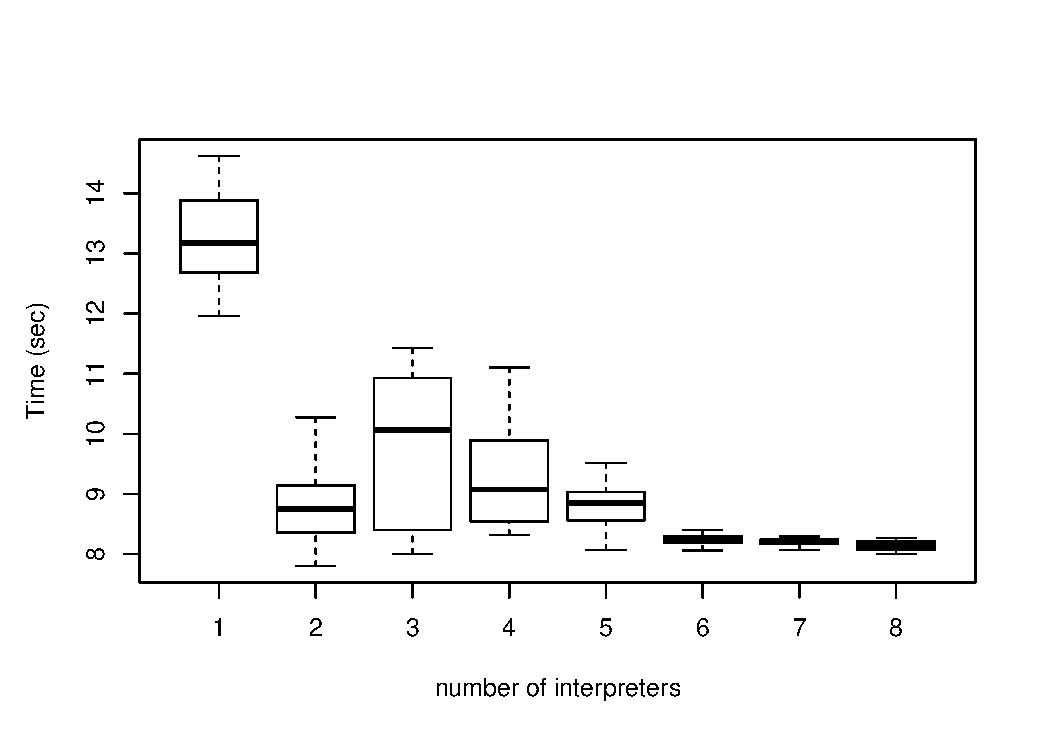
\includegraphics{rastrigin}
\caption{Диаграммы размаха времени исполнения
в зависимости от числа интерпретаторов}
\label{fig:rastriginboxplot}
\end{figure}

На рис.~\ref{fig:rastriginboxplot} видно,
что при увеличение числа интерпретаторов
время выполнения одной и той же задачи
описывает убывающую ветвь гиперболы.


\clearpage
\section*{Численные эксперименты}
\addcontentsline{toc}{subsection}{Численные эксперименты}

Тестирование проводилось на компьютере со следующими характеристиками:
\bigskip

\begin{tabular}{| c | c |}
    \hline
    Частота процессора & 3.7 ГГц \\ \hline
    Архитектура & 64-битная \\ \hline
    Модель процессора & Intel(R) Xeon(R) CPU E5-1620 v2 \\ \hline
    Число ядер & 8 \\ \hline
    Оперативная память & 64 Гб \\ \hline
    Объём жёсткого диска & 300 Гб \\
    \hline
\end{tabular}
\bigskip

Старой реализацией будем называть
изначальную реализацию,
где для вычисления функционала
на векторе параметров запускался
новый интерпретатор и
заново происходила загрузка
функции скрипта.

Новым вариантом реализации
будем называть реализацию,
где используется очередь задач
и пул потоков,
интерпретаторы инициализируются
один раз и не подвергаются перезапуску,
то есть время жизни интерпретатора
завершается с окончанием
вычислений функционала.

План тестирования заключался
в сравнение времени работы
старой и новой реализаций
при одинаковых параметрах.
Проводились многократные запуски
с целью подтверждения или опровержения
гипотезы о статистической значимости различий
времени работы реализаций.
Под нулевой гипотезой будет пониматься
различие математического ожидания
старой и новой реализаций.

Первым этапом численного эксперимента
было получение замеров времени
работы приложения
при различных комбинациях параметров.

Параметрами были выбраны следующие характеристики:

\begin{itemize}
    \item \textbf{Число потоков (\textit{i})}

        Для новой реализации этот параметр также
        обозначал размер пула потоков.
        Диапазон значений: 1-8.
    \item \textbf{Коэффициент размера популяции (\textit{M})}

        Размер популяции рационально выбирать
        пропорционально числу потоков,
        чтобы на каждый поток приходилась
        равная нагрузка при различном
        числе \textit{i}.

        Таким образом размер популяции равен:
        \begin{math}M * i\end{math}

        Тестирование проходило для значений:
        \begin{math}M = 5; M = 10\end{math}.
\end{itemize}

На следующих графиках представлены результаты тестирования:

% TODO

\includepdf[pages={-}]{zM10.pdf}

Было проверено, оказывает ли изучаемый параметр,
в данном случае это новый вариант реализации,
существенное влияние на интересующую нас
переменную, на время работы.
Проверка осуществлялась с помощью
критерия достоверно значимой
разности Тьюки
с уровнем значимости в 95\%.
Он необходим, чтобы посмотреть
где именно лежат статистические различия.

\bigskip
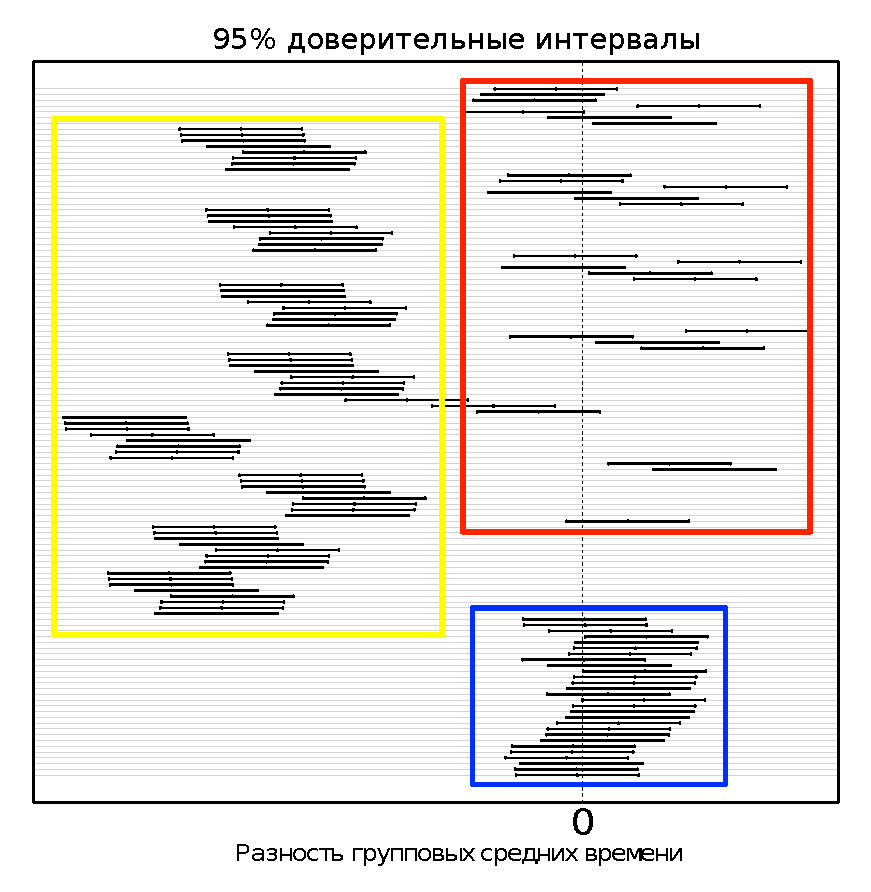
\includegraphics{tukey}

Пунктирной вертикальной линией показана
нулевая разница между групповыми средними времени.
Если доверительный интервал включает 0,
это указывает на отсутствие различий
между соответствующими группами.

На графике выделены три группы цветными рамками:
\begin{itemize}
    \item \textbf{Интервалы внутри красной рамки (справа вверху)} ---
        пары групп старой реализации с различным числом интерпретаторов.
        Интервалы лежат возле нуля, но присутствует
        некоторое разница, как в положительную сторону,
        так и в отрицательную. Это может объясняться
        конкуренцией интерпретаторов
        за вычислительные ресурсы и доступ к конфигурационным файлам
        при их одновременной инициализации.
    \item \textbf{Интервалы внутри синей рамки (справа внизу)} ---
        пары групп новой реализации с различным числом интерпретаторов.
        В данной группе различия минимальны,
        что является свидетельством оптимизации.
        В новой реализации инициализация интерпретаторов
        происходит единожды, поэтому
        узкое место не сильно замедляет работу
        при конкуренции, в дальнейшем
        интерпретаторы не так конкурируют за ресурсы.
    \item \textbf{Интервалы внутри жёлтой рамки (слева)} ---
        смешанные группы новой и старой реализации.
        Разница статистически значима,
        это означает, что оптимизация играет существенную роль.
\end{itemize}


\clearpage
\section*{Сегментация траекторий частиц}
\addcontentsline{toc}{subsection}{Сегментация траекторий частиц}

Обратной задачей математического моделирования
может являться выявление параметров взаимодействий биологических молекул,
которые не могут быть измерены напрямую из экспериментов.

Для тестирования программы использовалась
прикладная задача трэкинга частиц
и сегментации траекторий \cite{track}.

Исходными данными являются
серии снимков биологических макромолекул,
а именно эндосом эпидермального фактора роста
в клетках HeLa.

Первым этапом обработки происходит выделение
положения частиц из исходных снимков.
Затем с помощью стороннего программного обеспечения
производится построение траекторий.
Главной задачей является выяснить
как частицы движутся в клетке,
т.е. разбить траекторию на участки,
соответствующие либо диффузии,
либо направленному движению по микротрубочке.

Для последней задачи использовались
скрытые марковские модели,
что позволило получить
параметры движения и
построить вероятностную модель
биологического процесса.

Вероятности переходов и параметры движений
определяются из экспериментальных данных.
Скрипт для построения скрытой марковской модели
и использующий максимизацию правдоподобия
для определения параметров использует
метод ППРЭ и реализован на языке R.
Перед вычислением функционала качества
таблица траекторий подвергается предобработке.


\clearpage

\chapter*{ВЫВОД}
\addcontentsline{toc}{section}{ВЫВОД}

Работа развивает метод deep в направлении улучшения интеграции и это ведёт к увеличению проверки гипотез

TODO

\clearpage

\chapter*{ЗАКЛЮЧЕНИЕ}
\addcontentsline{toc}{section}{ЗАКЛЮЧЕНИЕ}

Целью работы было развитие метода ППРЭ,
путём улучшения интеграции
между методом оптимизации
и функционалом качества.
В результате исследования
предполагалось увеличить
эффективность реализованной
модификации метода ППРЭ
путём встраивания интерпретаторов
и экономии процессорного времени
на их инициализацию.

ППРЭ является методом
полностью параллельной разностной эволюции,
который используется для решения
обратной задачи математического моделирования.

Показана эффективность
оптимизации в сравнении с
прошлой реализацией.
Модификация ППРЭ
была разработана на основе
открытой кроссплатформенной
библиотеки GLib.

Полученная реализация
была протестирована на
прикладной задаче
сегментации траекторий частиц.
ППРЭ использовалась в этой задаче
для нахождения вероятностей переходов и
параметров движений
скрытой марковской модели по
экспериментальным данным.
В качестве тестовой фукции
также использовалась
смещённая функция Растригина.

Работа развивает метод deep
в направлении улучшения интеграции,
что ведёт к увеличению количества
проверяемых гипотез.


\clearpage

\bibliographystyle{utf8gost71u}
\bibliography{citations}

\end{document}

